\subsection{Techstack}
\setauthor{Zoe Emily Öllinger}

\begin{figure}[h]
    \centering
    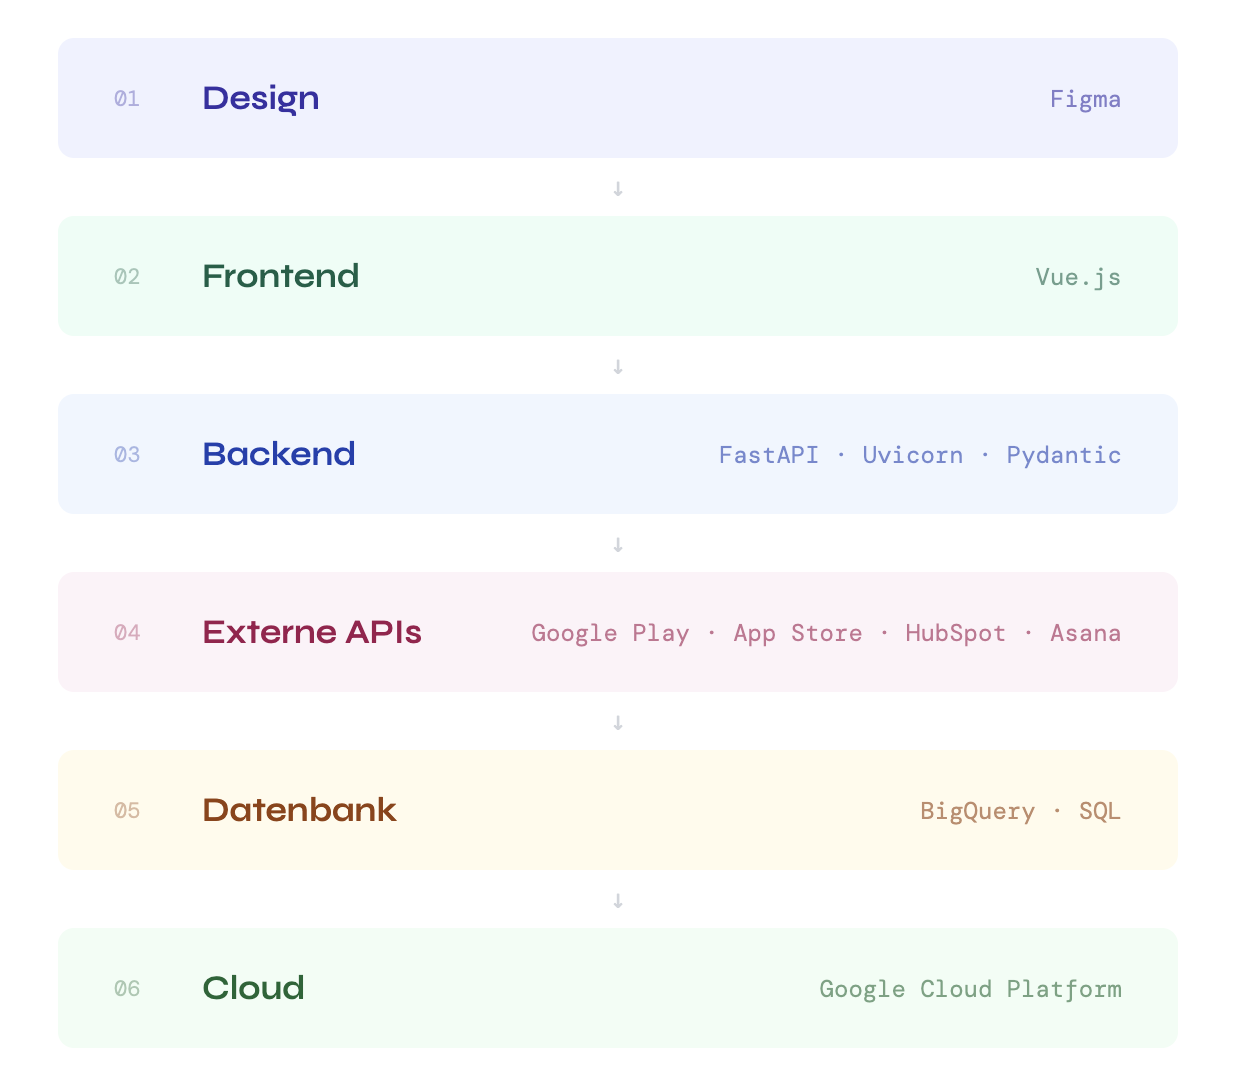
\includegraphics[width=0.8\textwidth]{pics/Techstack}
    \label{fig:Techstack}
\end{figure}

Der Techstack des Projekts lässt sich in sechs Schichten einteilen, die vom Design bis zur Cloud reichen.


\subsubsection{Design - Figma}
\setauthor{Zoe Emily Öllinger}

Bevor gecoded wurde, wurden die Konzepte, das Design und die Userexperience in Figma erarbeitet.
Im Projekt wurden damit sämtliche Ansichten des Health Monitoring Dashboards visuell erstellt, wie zum Beispiel die Layouts und das Farbschema sowie die Kommentaransicht und die Health-Checks.


\subsubsection{Frontend - Vue.js}
\setauthor{Zoe Emily Öllinger}

Die Benutzeroberfläche wurde mit Vue.js umgesetzt, einem JavaScript-Framework für die Entwicklung von Single Page Applications.
Jedes UI-Element, sowie die Filtertabs, die Übersichtstabelle oder der Detail-Button wurden als eigenständige, wiederverwendbare Komponente programmiert.


\subsubsection{Backend - FastAPI, Uvicorn, Pydantic, JavaScript}
\setauthor{Zoe Emily Öllinger}

Das Backend bildet den wichtigsten Part der Datenverarbeitung.
Als primäres API-Framework wurde FastAPI verwendet.

TODO: Elias checken und evtl ergänzen


\subsubsection{Externe APIs - Google Play, App Store Connect, HubSpot, Asana}
\setauthor{Zoe Emily Öllinger}

Es wurden mehrere externe Dienste über ihre APIs eingebunden.
Die Google Play Developer API und die App Store Connect API liefern Verfügbarkeits und Statusdaten.
Asana dient als Projektmanagement-Tool und liefert die im Dashboard sichtbaren Ticket und Task Zahlen der einzelnen Clients.
HubSpot wird als CRM-System eingebunden, um Kundenstammdaten abzurufen.

TODO: Elias checken ob i eh kan bledsinn gschriebn hob


\subsubsection{Datenhaltung - BigQuery, SQL}
\setauthor{Zoe Emily Öllinger}

Für die Speicherung großer Datenmengen wird Google BigQuery verwendet.
Die Abfragesprache SQL wird genutzt, um Datensätze wie MRR-Werte dem Backend zur Verfügung zu stellen.
TODO: Elias checki checki


\subsubsection{Datenhaltung - BigQuery, SQL}
\setauthor{Zoe Emily Öllinger}

Die Infrastruktur läuft auf der Google Cloud Platform.
GCP übernimmt Hosting, Deployment und den Betrieb des Backends.